\subsection{Use Case Diagram}

The GIS module Use Case requires an agent to be able to add GIS objects to the database. These objects contain both spacial data for their real life location, and attribute tables which contain the meta data about each object. \\

\begin{figure}[ht]
  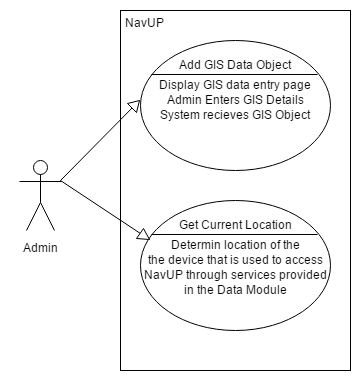
\includegraphics[width=0.8\textwidth]{GIS/GIS_Use_case.png}
\end{figure}

\subsection{State Diagram}
The GIS module is not a state dependant system. \\

\subsection{Sequence Diagram}

\subsection{Package Diagram}

\subsection{Activity Diagram}

\begin{figure}[ht]
	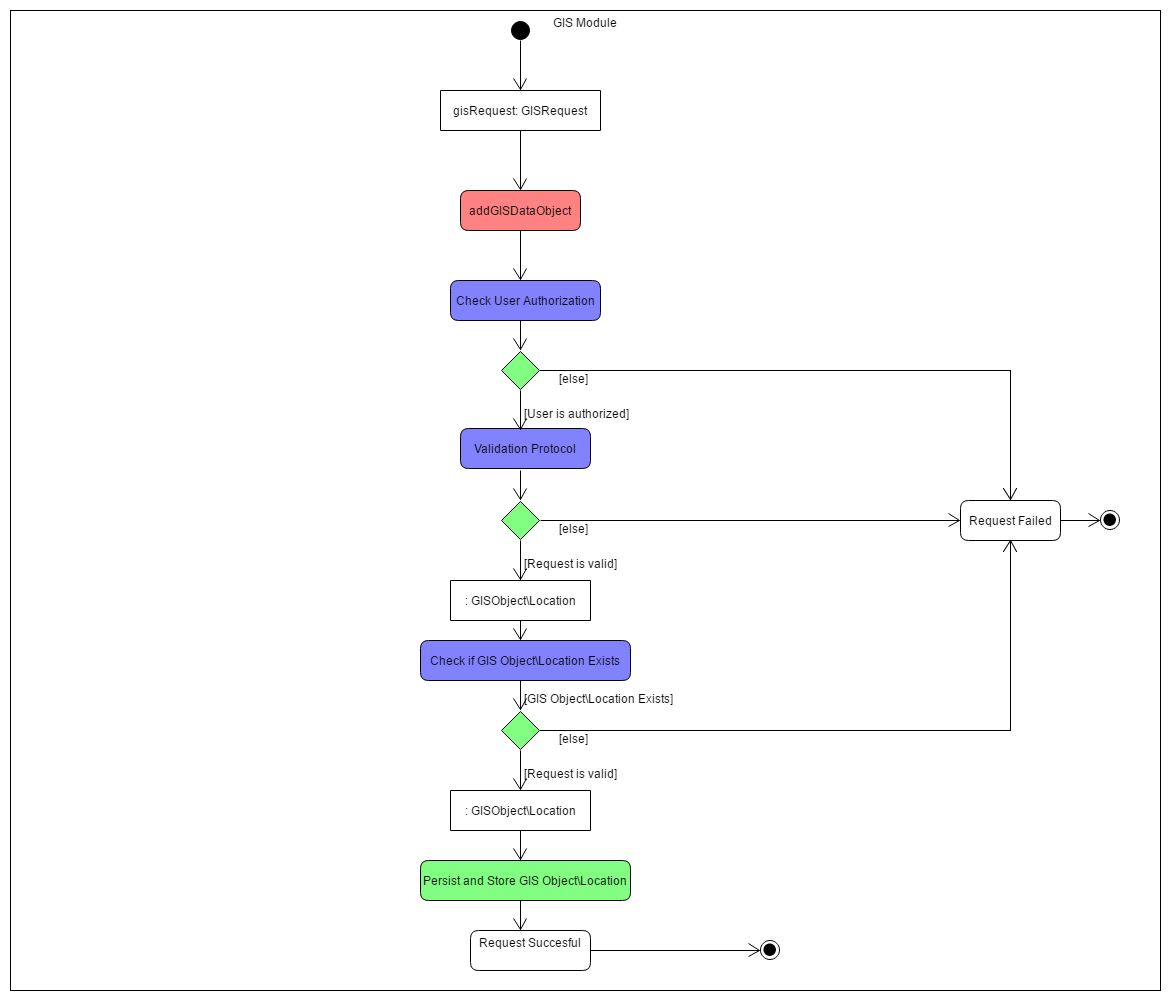
\includegraphics[width=0.8\textwidth]{GIS/GIS_Activity-addGISObject.png}
\end{figure}
\subsection{Class Diagram}

\begin{figure}[ht]
	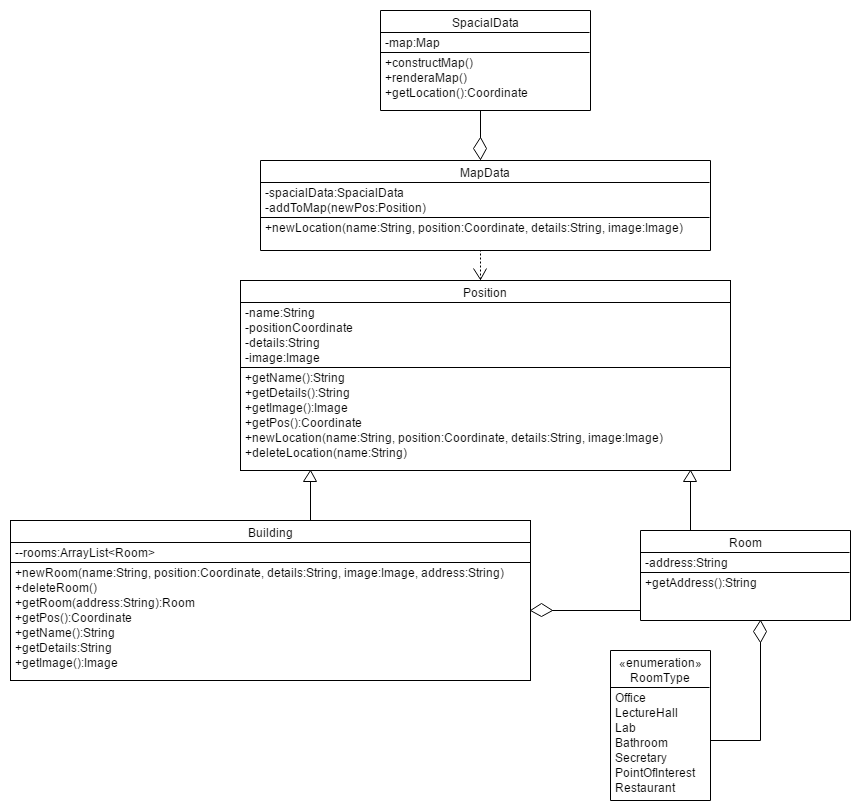
\includegraphics[width=0.8\textwidth]{GIS/GIS_Class_Diagram.png}
\end{figure}